\chapter{Results}
\label{chap:results}

% Qualitative first, as is the way in EDS.
% 	- spectrum calibrated, 5-30 kV
% 	- one plot for all
% 	- Look at energy scale for all results. How does the peaks deviate with the Ga As calibration?
% 	- Cu tape (give type) is not good as a Cu reference.
% 	- The stub is not Fe as expected, but Al. Makes sence, since steel is alloys and is magnetic.

% Quantitative
% 	- initial
% 	- background
% 	- peak fitting


% \section{Introduction}
% \label{sec:results:intro}
The results are presented in this chapter.
First qualitative then quantitative results are presented.
All the spectra taken were qualitatively analyzed.
Only the GaAs bulk spectra was quantitatively analyzed.
The spectrum from the GaAs bulk wafer taken on 30 kV is shown in \cref{fig:GaAs30kV_HS}.
This plot was made with HyperSpy, which utilize Matplotlib for plotting.
The plotting method in HyperSpy can add where the theoretical peak centers are.
The lines added also show an estimate of the weight of the peak.


% add figure figures/GaAs30kV_HS.png
\begin{figure}
    \centering
    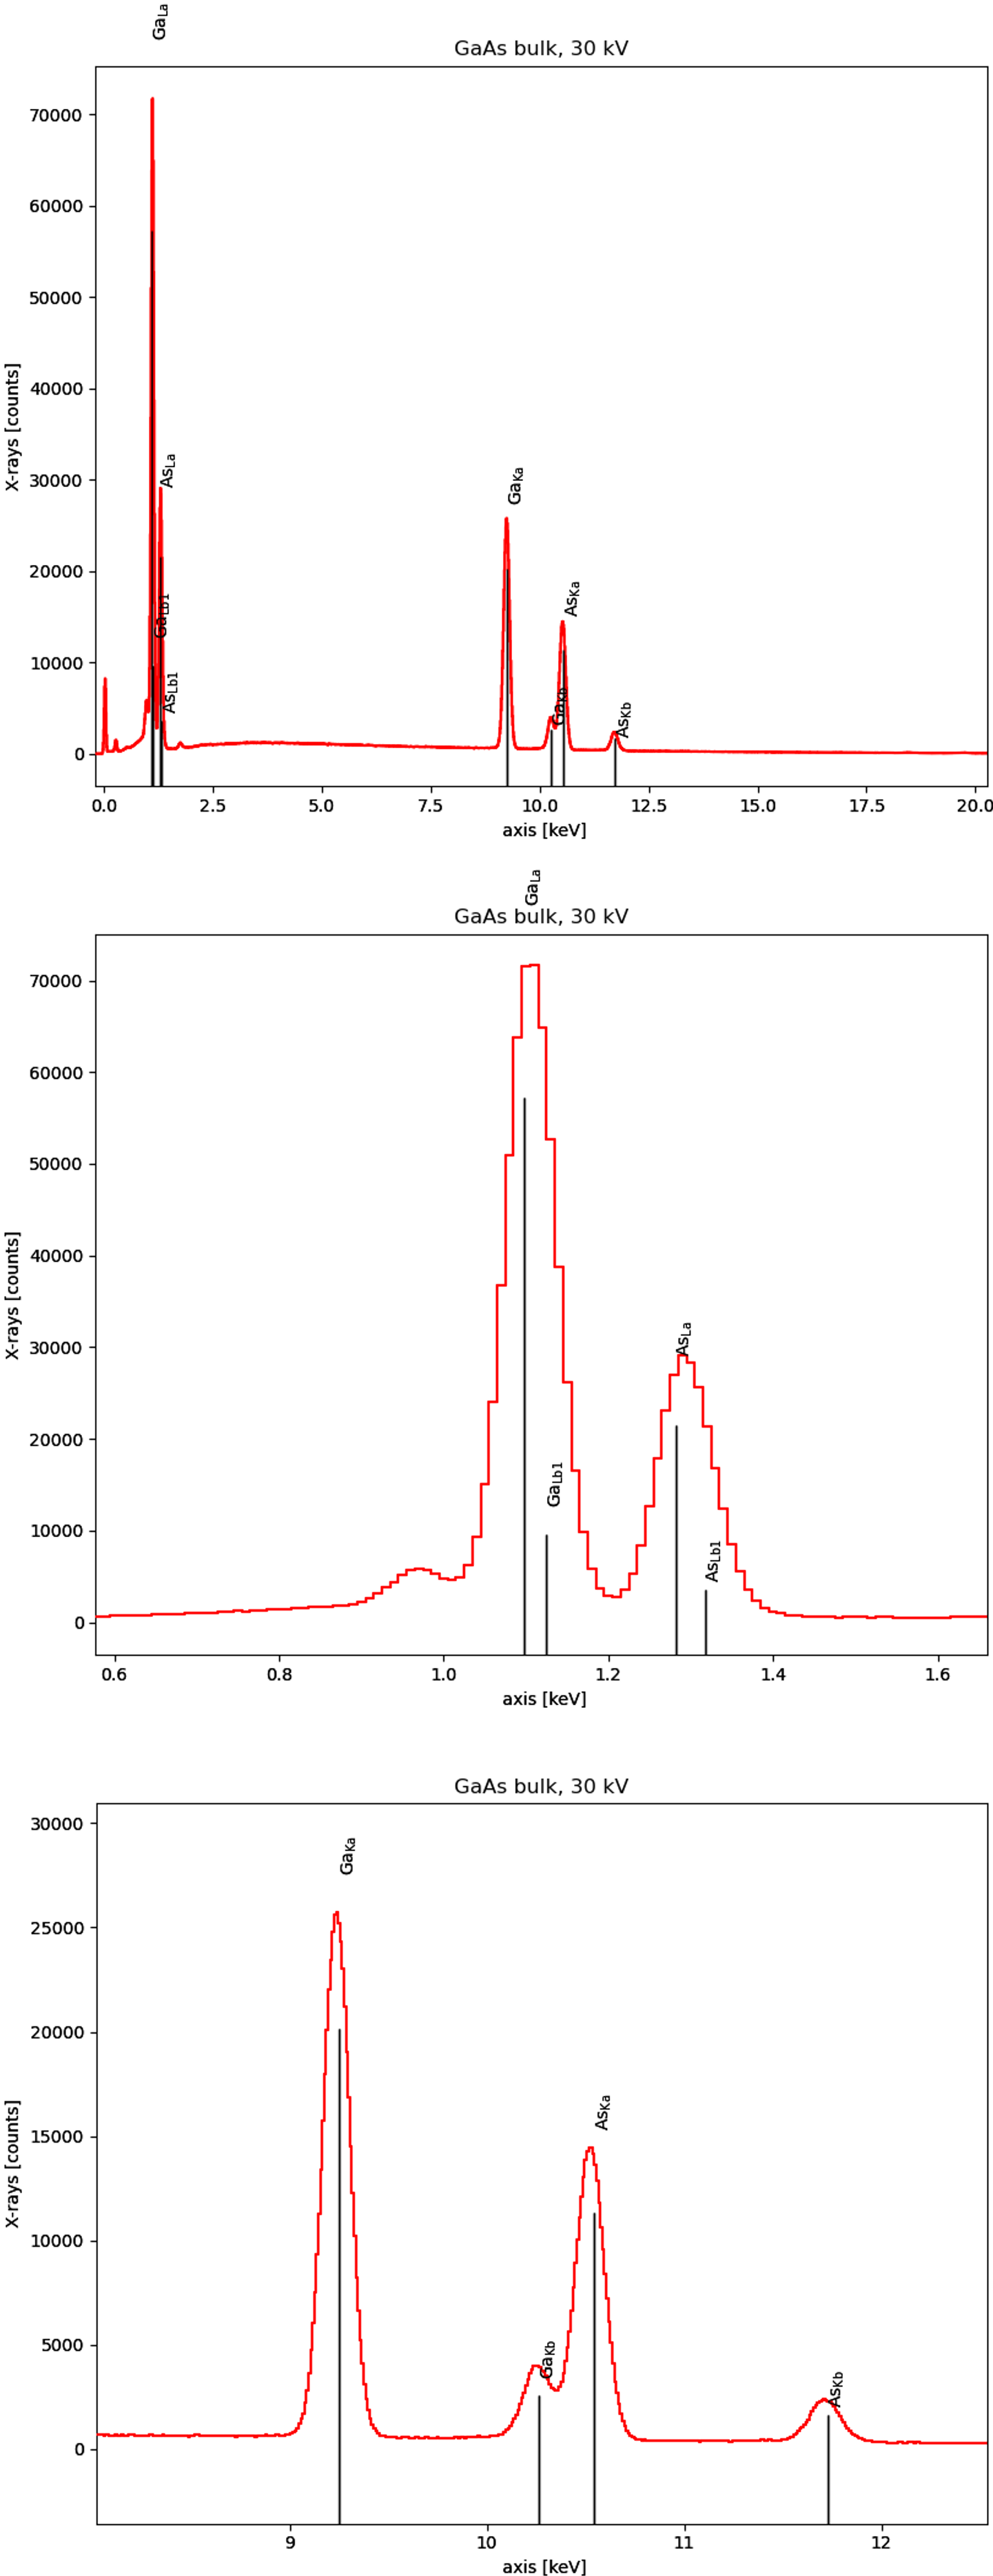
\includegraphics[width=0.90\textwidth]{figures/GaAs30kV_HS.png}
    \caption{
        The GaAs spectrum taken at 30 kV.
        This plot was made with HyperSpy, which use Matplotlib.
        The theoretical peak centers are added as lines.
        (a) is the whole spectrum.
        (b) is the zoomed in on the L-peaks.
        (c) is zoomed in on the K-peaks.
        (d) is zoomed in on the Ga K$\alpha$ peak.
        This plot has the calibration from AZtec, and it is clear that the line position is deviating from the center of the peaks.
    }
    \label{fig:GaAs30kV_HS}
\end{figure}




\section{Qualitative results}
\label{sec:results:qualitative}

\cref{fig:results:Spectra_Al} to \cref{fig:results:Spectra_Si} shows the spectra for the six different areas of the sample plotted with Plotly.
The plots are available as an interactive HTML plots on the GitHub repository.
\brynjar{Upload the HTML files to the GitHub repository.}
The calibration used in these spectra is based on the calibration of Ga L$\alpha$ and As K$\alpha$ from the GaAs bulk wafer.
The y-axis is normalized to the highest peak value in each spectrum.



% figures of the spectras

% figure Spectra_Al.png
\begin{figure}
    \centering
    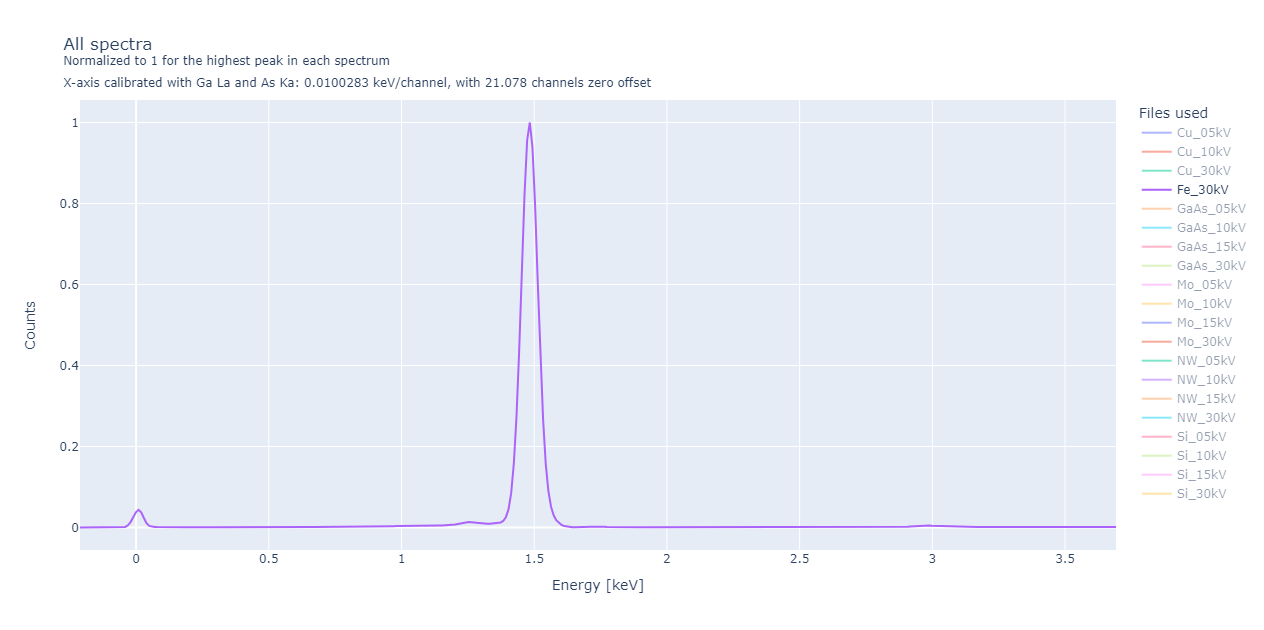
\includegraphics[width=0.70\textwidth]{figures/Spectra_Al.png}
    \caption{
        The spectra of the Al sample part.
        This was expected to be Fe, thus the label is wrong.
        The peak at 1.48 keV is the Al K$\alpha$ peak.
    }
    \label{fig:results:Spectra_Al}
\end{figure}

% figure Spectra_Cu.png
\begin{figure}
    \centering
    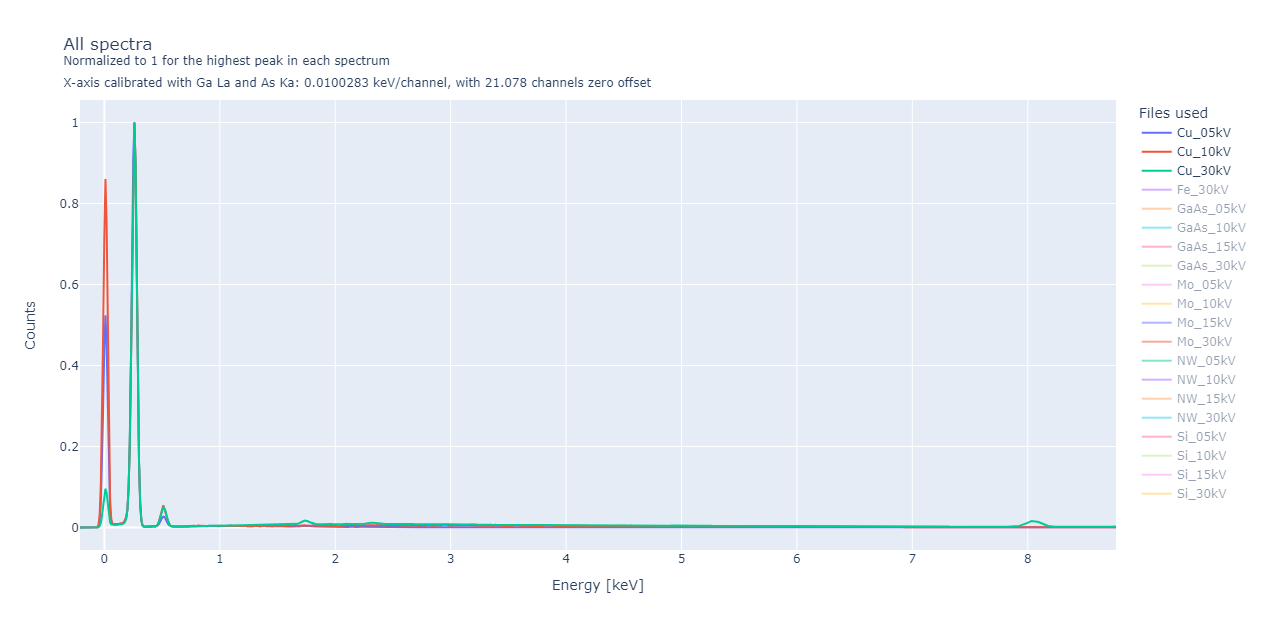
\includegraphics[width=0.70\textwidth]{figures/Spectra_Cu.png}
    \label{fig:Spectra_Cu}
    \caption{
        The spectra of the Cu sample part.
        The Cu sample was Cu-tape from the lab, but the Cu K$\beta$ peak is only barely visible at the 30 kV spectrum.
        The highest peak in all three spectra is at 0.260 keV, which is the C K$\alpha$ peak, slightly off from the expected 0.277 keV.
    }
\end{figure}

% figure Spectra_GaAs.png
\begin{figure}
    \centering
    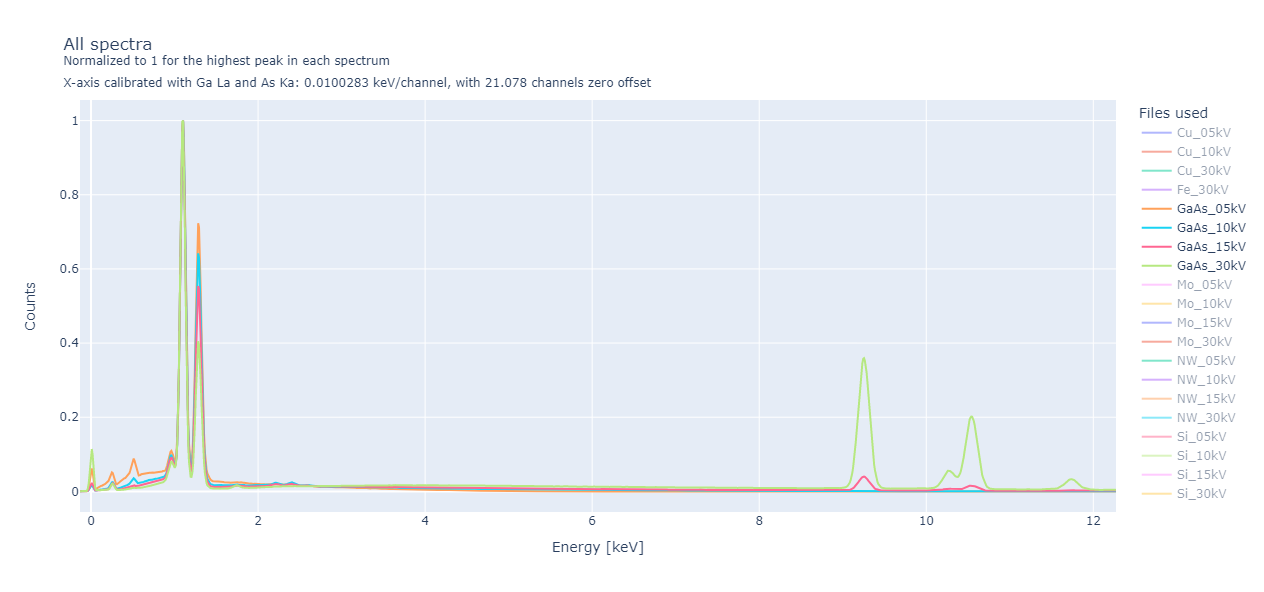
\includegraphics[width=0.70\textwidth]{figures/Spectra_GaAs.png}
    \label{fig:Spectra_GaAs}
    \caption{
        The spectra of the GaAs sample part.
        Both the K-peaks and the L-peaks of Ga and As are visible.
        There is a peak at 0.511 keV, which is the O K$\alpha$ peak.
        There is a peak at 0.260 keV, which is the C K$\alpha$ peak.
    }
\end{figure}

% figure Spectra_Mo.png
\begin{figure}
    \centering
    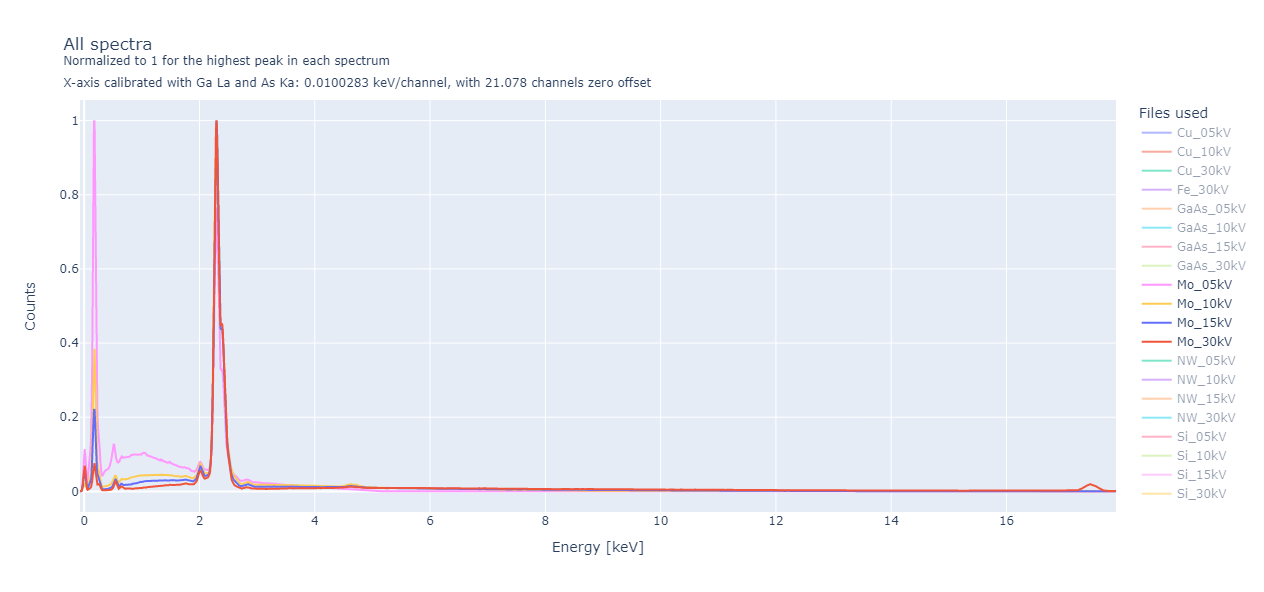
\includegraphics[width=0.70\textwidth]{figures/Spectra_Mo.png}
    \label{fig:Spectra_Mo}
    \caption{
        The spectra of the Mo sample part.
        The Mo K$\alpha$ peak at 17.47 keV is barely visible at the 30 kV spectrum, and has a high noise level.
        The high dobble peak is Mo L$\alpha$ at 2.29 keV and Mo L$\beta$ at 2.39 keV.
    }
\end{figure}

% figure Spectra_NW.png
\begin{figure}
    \centering
    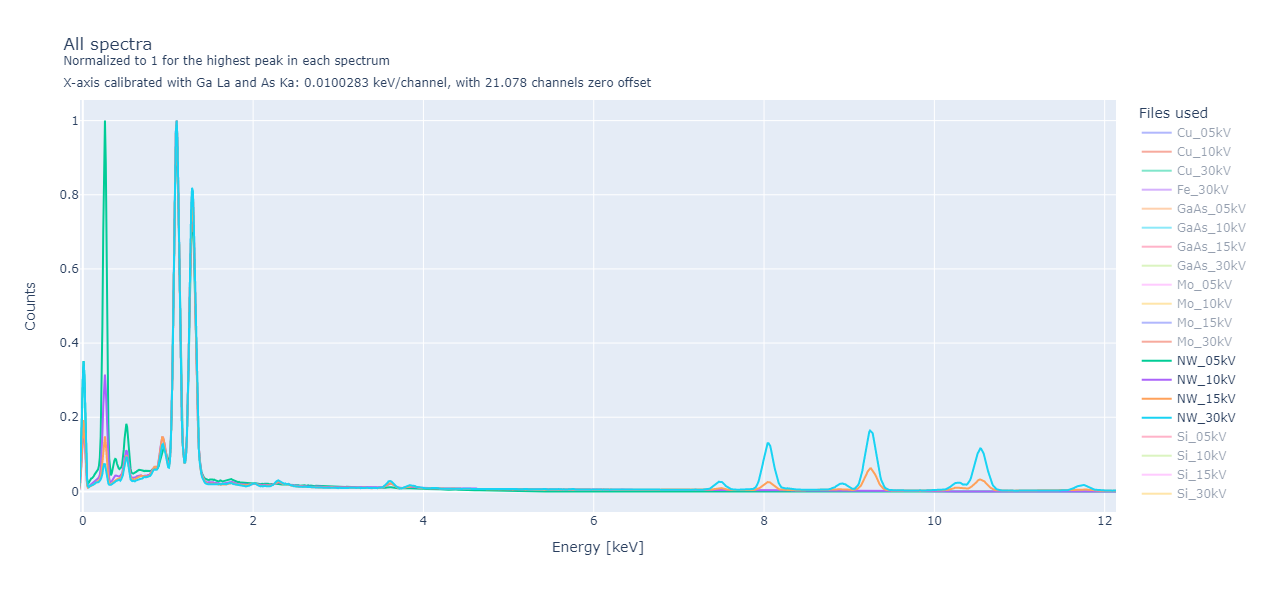
\includegraphics[width=0.70\textwidth]{figures/Spectra_NW.png}
    \label{fig:Spectra_NW}
    \caption{
        The spectra of the nanowire sample part.
        This spectrum have the most peaks, and contains Ga, As, Cu, Sb (? at 3.6 keV), Mo, C, and O.
    }
\end{figure}

% figure Spectra_Si.png
\begin{figure}
    \centering
    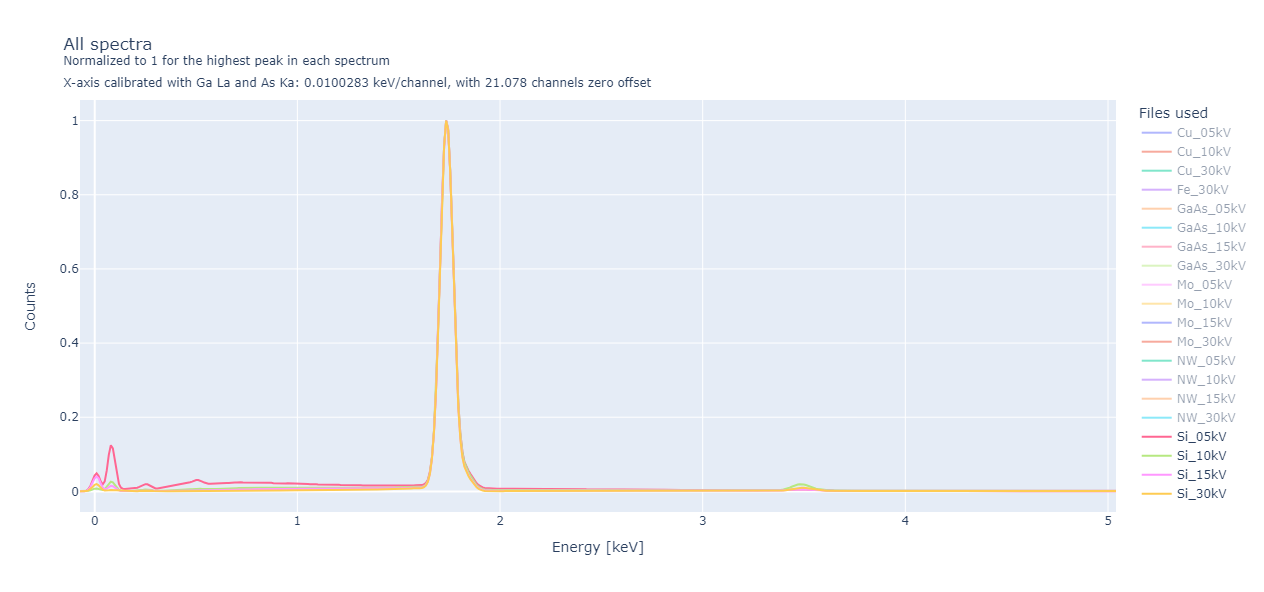
\includegraphics[width=0.70\textwidth]{figures/Spectra_Si.png}
    \label{fig:Spectra_Si}
    \caption{
        The spectra of the pure Si wafer sample part.
        All four spectra have one large peak at 1.73 keV, which is the Si K$\alpha$ peak.
        The four spectra also have a small peak at 3.48 keV, which is not identified.
    }
\end{figure}

\subsection{Peaks and background}
\label{sec:results:qualitative:peaks}
% Peaks, 
% zero peak
% peak width higher at higher E
% very strange that Cu 30 kV have a small Cu Ka and no Cu La at all (since La is bigger than Ka and Ga and Cu is close in the table), which is the case for Ga

All the spectra have peaks with high peak-to-background ratio.
The zero peak from the Oxford detector is visible in all the spectra as the first peak, with a center at 0.00924 keV.
The GaAs, NW and Mo spectra show clearly that the peaks broaden with higher E, since they have peaks at low and middle to high energy.
In all the spectra, the highest peaks are below 5 keV. % discussion: what peaks give the highest counts, with theory and empirical data. detector efficiency? Absorption? Overvoltage? etc
When doing the qualitative analysis, it became clear that the FIB stub was not made of Fe as expected, but rather of Al with a peak at 1.48 keV.
The FIB stub have a small peak at 1.25 keV, which could be from Mg K$\alpha$ at 1.253 keV.
The Al FIB stub spectrum also have a small peak at 5.90 keV, which could be from Mn K$\alpha$ at 5.899 keV.
% discussion: Al-Mg-Mn alloy, but unable to quantify with my bad signal, or?
Another discovery was that the Cu-tape does not give a good Cu signal.
The high peak in the Cu-tape spectra at 0.260 keV are from C and not the Cu L$\alpha$ peak.
Only the Cu-tape taken at 30 kV has a Cu peak, but it is very small.
Even though the Cu spectra at 30 kV has the Cu K$\alpha$ peak, the Cu L$\alpha$ peak is completely missing. % this is very, very strange. ! TODO: Discuss
\brynjar{add transition sentence.}

% double peaks, ie peaks which are overlapping
Some of the peaks in the spectras are overlapping, which shifts the shape of the peaks.
An example of this is the As K$\alpha$ peak and the Ga K$\beta$ peak in the GaAs bulk wafer spectra.
These peaks are overlapping, but also far enough apart that the peaks are still distinguishable.
Another example of overlapping peaks is the Mo L$\alpha$ peak and the Mo L$\beta_1$, which are overlapping so much that they are hard to distinguish.
Since they are harder to distinguish, the peak fitting makes one Gaussian for the two peaks, which is off on both peak centers. % for discussu\ion: which is why the deviation of the Mo L$\alpha$ peak is off in the calibration accuracy table, \cref{tab:results:calibration-peak-accuracy}.
Overlapping peaks makes counting the signal from spesific peaks harder.
\brynjar{Figure of double peaks?}


The signal from the background is another factor which makes counting more difficult.
In general, background in the aquired spectra is low, but with different shapes.
In the GaAs, Si and Mo the height of the background decrease with higher acceleration voltage.
In the Cu spectra the background increase with higher acceleration voltage.
In the NW spectra the background is fairly similar, except for the 5 kV spectrum where the background is cut off at 5 keV.
All the 5 kV spectra decrease more or less linearly from 1 to 5 keV. % discusiion: overvoltage
The background is very low and almost flat above the highest peak in the spectra. % discussion: nothing to reduce the speed of the e-
For example, the Cu 10 kV spectrum have its highest peak at 0.5 keV, and the background is almost flat above 0.5 keV.
The background in the Si 30 kV spectrum increase a lot up to the high Si K$\alpha$ peak at 1.7 keV, and then the background drops down right after the peak.
The background in Si 30 kV is 10 times higher before than after the peak, and does also have a different shape before and after the peak at 1.7 keV.
The background shape in Si 30 kV is almost linear from 0.6 to 1.6 keV, drops down to 10\% height from 1.6 to 1.9 keV, and then follows the expected background shape from 1.9 keV.
The expected background shape is illustrated in \brynjar{Make a drawing of the background.} % discussion: explain that the bg is dependent on a peak (ie material) being present. This makes fiting hard, since there are some peak-dependency which is hard to predict.
%discussion: model the peak as more than one polygon added together, since the shape changes. For further works. That is called spline.
All the other spectra show the same behavior with their heighest peak and the peaks affect on the background as the Si 30 kV spectrum.
In general, the background singals are low, but their different shapes and heights makes it harder to fit the peaks of the characteristic X-ray lines.
\brynjar{Figure of background? And figure of fit of background before and after a tall peak?}
\ton{The last sentence is meant to be a transition/finishing sentence, but might be too much discussion.}

% background, 
% bg increase with lower kV, 
% bg shape, 


% \subsection{Spectra artifacts and strays}
% \label{sec:results:qualitative:artifacts}

% Use time on this to show that I have results and that I know what I am doing.
% It will also help to point at errors in AZtec.

In addition to the characteristic peaks and the background, there are also artifacts and strays in the spectra. % discussion: lower peaks are super important, eg in the Al spectra where it is small amounts of Mg and Mn, probably. Asserting what is a stray and what is characteristic is important for quantification.
All the spectra have a Si peak at 1.74 keV. % This is the Si escape peak for some spectra, but not all.
Some of the spectra have peaks from areas outside the impacted area of the main beam, like the Mo, Sb and Cu peak in the NW spectra. % pretty sure it is Sb, because of the series of peaks at 3.6, 3.8, 4.1 and 4.3. 
% discuss both interactin volume and bonus peaks from X-ray strays in the chamber/sample.
The Sb peaks in the NW spectra are at 3.60, 3.85, 4.10 and 4.35 keV, being the L$\alpha_1$, L$\beta_1$, L$\beta_2$ and L$\gamma_1$ peaks.
NW have clear C K$\alpha$ and O K$\alpha$ peaks ar 0.260 and 0.515 keV.
GaAs and Mo have some C and O signal.
The C and O signal is higher at lower acceleration voltage.
All four Mo spectra have a peak at 0.175 keV, which match with B K$\alpha$ or Be K$\alpha$.
% discussion: understanding the strays properly is actually helpful for the qualitative analysis, since some elements can be excluded based on the strays and some strays are only present in certain materials.
% Si stray in all spectra
% stray in NW outside beam, Mo, Cu and Sb

Another aritfact present in most spectra is sum peaks.
The Si spectra have a sum peak at 3.49 keV, which is the sum of Si K$\alpha$ at 1.74 keV. % discusiion: this could be Sb, but not like NW where Sb is a series of peaks. Also say something about the resolution of the detector, which is higher at lower E. And also that Sb cannot be excluded bc. of the K peak. And also that the sum peaks can be tested with low DT. And something here about the bad calibration in AZtec which might make this sum peak as a Sb peak, but I now know that it is a Si peak sum peak and not a Sb peak.
The Al spectrum have its highest peak at 1.48 keV and a sum peak at 2.98 keV
The Mo spectrum have a sum peak at 4.65 keV, which is the sum of Mo L$\alpha$ at 2.293 keV and Mo L$\beta_1$ at 2.395 keV. % same shape as Mo La  Mo Lb1, i.e. also Mo La+MoLa sum
The GaAs spectrum at 30 kV have two small sum peak signals at 18.5 and 19.5 keV, while the NW spectrum at 30 kV with lower DT does not have these peaks. % discussion: results show that sum peaks are lower with lower DT

% Mo double peak
% GaAs double peak
% Si stray on Cu
% also a sum peak at Al 30 kV spectrum (look at DT)
% Si double count at 3.4 keV which could be Sn (but the E resolution could seperate them Ton thinks at this low keV and Sn would have multiple peaks, cannot exclude bc of the K peak could count with low DT to minimize double counts consequence of AZtecs bad calibration)



\subsection{Calibration}
\label{sec:results:qualitative:calibration}

% what I did to calibrate the spectra
Different calibrations were explored.
The initial calibration is the one from AZtec, and is the one used in the spectra in \cref{fig:GaAs30kV_HS}.
This calibration has a left shift for the L-peaks and a right shift for the K-peaks.
The second type of calibration is the one given by the model fit in HyperSpy.
The third type is from the self made model fit, using the distance between two high intensity and far apart peaks to calibrate the energy scale.
The third type is both calculated with the Ga L$\alpha$ and As K$\alpha$ peaks in the GaAs 30 kV spectrum, and with Mo L$\alpha$ and Mo K$\alpha$ peaks in the Mo 30 kV spectrum.

% the values
Values for the four calibrations are given in \cref{tab:results:calibrations}.
The deviations are a few percent, and the accuracy of the different calibrations give on spesific peaks are given in \cref{tab:results:calibration-peak-accuracy}.
Here accuracy is the difference between the theoretical peak position and the peak center in the spectrum, given in percent.
For almost all the peaks, the deviation is greatest for the AZtec calibration.
One exception is the C K$\alpha$ peak, which deviates a lot less for the AZtec calibration. %discussion: Aztec might use the zero peak to calibrate, but that is just speculation.
The difference between the HyperSpy calibration and the self made calibration on the GaAs and Mo spectra are small.
In the following qualitative section, the effect of the different calibrations on the spectra are presented.

% dispersion and offset table
% Calibration values
% chapter Results
\begin{table}[ht]
    \centering
    \caption{
        Different calibration values.
        The AZtec calibration is reffered to as the uncalibrated value.
        The dispersion is calculated with \cref{eq:theory:calibration:dispersion}.
        The offset is calculated with \cref{eq:theory:calibration:offset}.
        The own calibration was done on Ga L$_\alpha$ and As K$_\alpha$ from the 30 kV measurement on the GaAs wafer.
        The HyperSpy cailbration was done by making a model and fitting it to the data on the 30 kV GaAs spectrum.
    }
    \label{tab:results:calibrations}
    % \begin{tabular}{m{4cm} m{2cm} m{2cm}}
    \begin{tabular}{ccc}
        Calibration method & Dispersion,   & Zero offset \\
                           & [keV/channel] & [channels]  \\
        \hline
        AZtec              & 0.01          & 20          \\
        HyperSpy           & 0.010028      & 21.0787     \\
        Own calibration    & 0.010030      & 21.127
    \end{tabular}
\end{table}


% calibration peak accuracy table
% table with peak accuracy

\begin{table}[p]
    \centering
    \caption{
        % TODO: give the peak accuracy in ev, not percent. Or eV and percent?
        Peak accuracy of the different calibration methods on 30 kV spectra: NW, Mo, Si, Al, Cu. % TODO: reformulate
        The other acceleration voltages gave similar results.
        The accuracy here is the deviation from the theoretical peak to the measured peak.
        The percentage deviation is also given.
        The measured peak is the fitted center of the peak.
        % discussion: The Mo L$\alpha$ deviates much because the peak is not well fitted.
        % The C K$\alpha$ is fitted well, but deviates much more than all the other peaks.
        The self-made calibration was done on two spectra: GaAs and Mo. % discussion: Mo is more far apart than GaAs.
        % One was done on Ga L$\alpha$ and As K$\alpha$ from the 30 kV measurement on the GaAs wafer.
        % The other was done on the more far apart peaks Mo L$\alpha$ and Mo K$\alpha$ from the 30 kV measurement on the Mo wafer.
        The HyperSpy calibration was done on the GaAs spectrum.
        At the bottom the RMS of the deviation in the column is given.
    }
    \label{tab:results:calibration-peak-accuracy}
    \begin{tabular}{cccccc}
        Peak         & Theoretical & AZtec                 & HyperSpy              & Ga L$\alpha$ \& As K$\alpha$ & Mo L$\alpha$ \& Mo K$\alpha$ \\
                     & [keV]       & [eV]                  & [eV]                  & [eV]                         & [eV]                         \\
        \hline
        As L$\alpha$ & 1.2819      & 12.8,\,\,\,    1.0\%  & 5.6,\,\,\,    0.4\%   & 5.4,\,\,\,    0.4\%          & 7.2,\,\,\,    0.6\%          \\
        As K$\alpha$ & 10.5436     & -21.3,\,\,\,   -0.2\% & -2.7,\,\,\,   -0.0\%  & -1.1,\,\,\,   -0.0\%         & 9.8,\,\,\,    0.1\%          \\
        Ga L$\alpha$ & 1.098       & 11.5,\,\,\,    1.0\%  & 3.8,\,\,\,    0.3\%   & 3.5,\,\,\,    0.3\%          & 5.1,\,\,\,    0.5\%          \\
        Ga K$\alpha$ & 9.2517      & -14.2,\,\,\,   -0.2\% & 0.9,\,\,\,    0.0\%   & 2.2,\,\,\,    0.0\%          & 11.9,\,\,\,    0.1\%         \\
        Cu L$\alpha$ & 0.9295      & 16.4,\,\,\,    1.8\%  & 8.3,\,\,\,    0.9\%   & 8.0,\,\,\,    0.9\%          & 9.4,\,\,\,    1.0\%          \\
        Cu K$\alpha$ & 8.0478      & -9.2,\,\,\,   -0.1\%  & 2.5,\,\,\,    0.0\%   & 3.7,\,\,\,    0.0\%          & 12.1,\,\,\,    0.2\%         \\
        Mo K$\alpha$ & 17.4793     & -56.8,\,\,\,   -0.3\% & -18.8,\,\,\,   -0.1\% & -15.8,\,\,\,   -0.1\%        & 1.9,\,\,\,    0.0\%          \\
        Mo L$\alpha$ & 2.2932      & 24.0,\,\,\,    1.0\%  & 19.7,\,\,\,    0.9\%  & 19.7,\,\,\,    0.9\%         & 22.5,\,\,\,    1.0\%         \\
        Si K$\alpha$ & 1.7397      & 2.9,\,\,\,    0.2\%   & -3.0,\,\,\,   -0.2\%  & -3.2,\,\,\,   -0.2\%         & -1.0,\,\,\,   -0.1\%         \\
        Al K$\alpha$ & 1.4865      & 3.0,\,\,\,    0.2\%   & -3.7,\,\,\,   -0.2\%  & -3.9,\,\,\,   -0.3\%         & -1.9,\,\,\,   -0.1\%         \\
        Cu K$\alpha$ & 8.0478      & -9.3,\,\,\,   -0.1\%  & 2.4,\,\,\,    0.0\%   & 3.5,\,\,\,    0.0\%          & 11.9,\,\,\,    0.1\%         \\
        C K$\alpha$  & 0.2774      & -8.2,\,\,\,   -3.0\%  & -18.3,\,\,\,   -6.6\% & -18.7,\,\,\,   -6.7\%        & -17.9,\,\,\,   -6.5\%        \\
        \hline
        RMS  [eV]    &             & 14.75                 & 4.62                  & 4.55                         & 9.57
    \end{tabular}
\end{table}









\section{Quantitative results}
\label{sec:results:quantification}

% from intro paragraph:
% The different methods are using AZtec and two approaches in HyperSpy.
% The different adjustments are results with different calibrations, different background models, \brynjar{"and different peak models"?}


% \subsection{Quantification methods}
% \label{sec:results:quantification_methods}
% How accurate it the out-of-the-box quantification in AZtec and HyperSpy?

% Its okay to only do the GaAs here.
% Could also look at NW, but not nessesary.

To do the quantitative analysis, HyperSpy needs k-factors.
The k-factors for Ga and As are given in \cref{tab:results:k-factors}.
These k-factors are from the GaAs bulk wafer, and HyperSpy have estimated them theoretically.
\ton{Shall I list the other k-factors for the other sample areas? I do not think I will use them, since I've only quantified the GaAs bulk wafer. But the other k-factors are results too. Eventually including NW data too, but I do not know that ratio.}

% table with the k-factors.
% Vacc, element, line, k-factor

\begin{table}
    \centering
    \caption{
        K-factors for Ga and As, extracted from AZtec.
        All the k-factors are theoretically estimated.
        AZtec provides either the k-factor for the L$\alpha$ or the K$\alpha$ line, and selects automatically based on the energy of the incident electrons.
    }
    \label{tab:results:k-factors}
    \begin{tabular}{cccc}
        V$_\textnormal{acc}$ [kV] & Element & Line      & K-factor \\
        \hline
        5                         & Ga      & L$\alpha$ & 1.086    \\
        5                         & As      & L$\alpha$ & 1.210    \\
        10                        & Ga      & L$\alpha$ & 1.223    \\
        10                        & As      & L$\alpha$ & 1.310    \\
        15                        & Ga      & L$\alpha$ & 1.259    \\
        15                        & Ga      & L$\alpha$ & 1.331    \\
        30                        & Ga      & K$\alpha$ & 3.268    \\
        30                        & As      & K$\alpha$ & 4.191
    \end{tabular}
\end{table}

The initial quantification was done on the data from the GaAs wafer in AZtec and in HyperSpy as out-of-the-box as possible.
The results are presented in \cref{tab:initial_quantification}.
The wafer is a 1:1 alloy of gallium and arsenic, so the atomic percent of Ga and As should be 50\% and 50\% respectively.

% initial quantification
% chapter Results
\begin{table}[ht]
    \centering
    \caption{
        Initial quantification of the GaAs wafer.
        The ratio in the wafer is 1:1, so the correct ratio is 50\% and 50\%, because the results are in atomic percent.
        \brynjar{Put in the actual results here. Use both HyperSpy linear and model fitted results?}
    }
    \label{tab:initial_quantification}
    \begin{tabular}{m{1.5cm} m{1.5cm} m{1.5cm} m{1.5cm} m{1.5cm}}
        $V_\textnormal{acc}$ & AZtec &       & HyperSpy &       \\
                             & Ga    & As    & Ga       & As    \\
        \hline
        5 kV                 & 50 \% & 50 \% & 50 \%    & 50 \% \\
        10 kV                & 50 \% & 50 \% & 50 \%    & 50 \% \\
        15 kV                & 50 \% & 50 \% & 50 \%    & 50 \% \\
        30 kV                & 50 \% & 50 \% & 50 \%    & 50 \%
    \end{tabular}
\end{table}


To better understand the ratios between Ga and As, the areas under the peaks in the spectra were counted.
Table \cref{tab:results:ratios} gives the ratios between the areas under the peaks for 5, 10, 15 and 30 kV.
The table compares L$\alpha$ peaks, K$\alpha$ peaks, K$\beta$ peaks and the sum of the peaks.
The table also lists the FWHM of the peaks.

\begin{table}[ht]
    \centering
    \caption{
        Ratios of Ga and As on the GaAs wafer, with the CLiff-Lorimer quantification raito.
        % The spectrum was calibrated with GaAs 30 kV.
        K$\beta$ at 15 kV was too low to be detected and is therefore not included in the table.
        The \emph{ratio} column is \emph{Ga sum} divided by \emph{As sum}.
        The \emph{CL} column is the CL quantification, done by multiplying the \emph{ratio} with $k_\textnormal{GaAs}$, from \cref{tab:results:k-factors}.
        The empty cells are for peaks where the was no k-factor or for the sum of the peaks, which have no center and no FWHM.
    }
    \label{tab:results:ratios}
    \begin{tabular}{ccccccccc}

        Peak                         & CL    & Ratio & Ga center & As center & Ga FWHM & As FWHM & Ga sum  & As sum \\
                                     &       &       & [keV]     & [keV]     & [eV]    & [eV]    &         &        \\
        \hline
                                     &       &       &           &           &         &         &         &        \\

        5 kV                         &       &       &           &           &         &         &         &        \\
        L$\alpha$                    & 1.151 & 1.282 & 1.101     & 1.288     & 74.010  & 80.921  & 75.462  & 58.844 \\
        \hline
                                     &       &       &           &           &         &         &         &        \\
        10 kV                        &       &       &           &           &         &         &         &        \\
        L$\alpha$                    & 1.349 & 1.444 & 1.100     & 1.287     & 73.841  & 80.827  & 76.222  & 52.770 \\

        \hline
                                     &       &       &           &           &         &         &         &        \\
        15 kV                        &       &       &           &           &         &         &         &        \\
        L$\alpha$                    & 1.579 & 1.669 & 1.100     & 1.287     & 73.830  & 81.137  & 77.001  & 46.146 \\
        K$\alpha$                    &       & 2.445 & 9.253     & 10.536    & 155.080 & 181.951 & 6.013   & 2.459  \\
        % K$\beta$       & 1.000 & 10.536         & 10.536         & 181.951      & 181.951      & 2.459   & 2.459  \\
        L$\alpha$+K$\alpha$          &       & 1.708 &           &           &         &         & 83.014  & 48.605 \\
        % L$\alpha$+K$\alpha$+K$\beta$ & 1.674 &            &            &          &          & 85.473  & 51.065 \\

        \hline
                                     &       &       &           &           &         &         &         &        \\
        30 kV                        &       &       &           &           &         &         &         &        \\
        L$\alpha$                    &       & 2.279 & 1.098     & 1.287     & 72.309  & 80.849  & 76.465  & 33.546 \\
        K$\alpha$                    & 1.301 & 1.678 & 9.253     & 10.542    & 157.799 & 168.238 & 58.718  & 34.994 \\
        K$\beta$                     &       & 1.603 & 10.276    & 11.736    & 171.804 & 185.034 & 8.821   & 5.503  \\
        L$\alpha$+K$\alpha$          &       & 1.972 &           &           &         &         & 135.184 & 68.540 \\
        L$\alpha$+K$\alpha$+K$\beta$ &       & 1.945 &           &           &         &         & 144.004 & 74.042
    \end{tabular}
\end{table}



One of the adjustments explored was the affect of the calibration on the quantification.
Using different the calibrations in \cref{tab:results:calibrations} gave different quantification results when using Cliff-Lorimer in HyperSpy. % discussion: Issue with using Clif-Lorimer since I have bulk and not thin sample.
The results are presented in \cref{tab:results:calibration-quantification}.
The quantification on 10 and 15 kV are obviously wrong, but the same method was used for all the  quantifications.




% table with peak accuracy

\begin{table}[ht]
    \centering
    \caption{
        Quantification with different calibration methods.
        The quantification is done by in HyperSpy with Cliff-Lorimer method.
        The CL method is for this samples, while the GaAs wafer used here is a bulk sample.
        AZ is the AZtec calibration.
        HS is the HyperSpy calibration.
        GaAs is the calibration on the GaAs 30 kV spectrum.
        The accuracy of the quantification is the deviation from 50\%, because the sampled area is 1:1 GaAs wafer.
    }
    \label{tab:results:calibration-quantification}
    \begin{tabular}{cccccc}
        Vacc & Element & Line & AZ     & HS     & GaAs   \\
        \hline
        5    & As      & L    & 44.81  & 44.29  & 44.19  \\
        5    & Ga      & L    & 55.19  & 55.71  & 55.81  \\
        10   & As      & L    & 100.00 & 100.00 & 100.00 \\
        10   & Ga      & L    & 0.00   & 0.00   & 0.00   \\
        15   & As      & L    & 5.23   & 4.39   & 5.87   \\
        15   & Ga      & L    & 94.77  & 95.61  & 94.13  \\
        30   & As      & K    & 56.25  & 57.14  & 59.02  \\
        30   & Ga      & K    & 43.75  & 42.86  & 40.98
    \end{tabular}
\end{table}

% affect of calibration
% accuracy on quantification


% affect of peak and background modelling
% both errors and the quantification accuracy
% could model as other than Gaussian? Discusssion




% Conclusion: update dispersion and offset for the APREO?